\section{Diseño de la Plataforma}
\thispagestyle{plain}

\vspace{0.5cm}

\Large\scshape
\begin{center}
    \textrm{Diseño de los circuitos principales y auxiliares de la plataforma}
\end{center}
\normalfont
%\normalsize

\divider

Si bien con el análisis del anterior capítulo se pudo conseguir un panorama general del funcionamiento de la plataforma, se presentan otras complejidades a la hora de plasmarlo en un sistema real: se requieren múltiples circuitos auxiliares además de los bloques principales (por ejemplo circuitos de adquisición de señales); aparecen consideraciones de diseño que no existen en el plano teórico; entre otras cuestiones. Este capítulo está dedicado al diseño real de la plataforma completa para luego implementar en una placa de circuito impreso o PCB, teniendo en cuenta estas complicaciones.\\

En la siguiente figura se muestra un diagrama detallado de la plataforma, dónde se presentan todos los distintos bloques funcionales, incluyendo los bloques auxiliares que no se trataron en el análisis del anterior capítulo.\\

\begin{figure}[h]
    \centering
    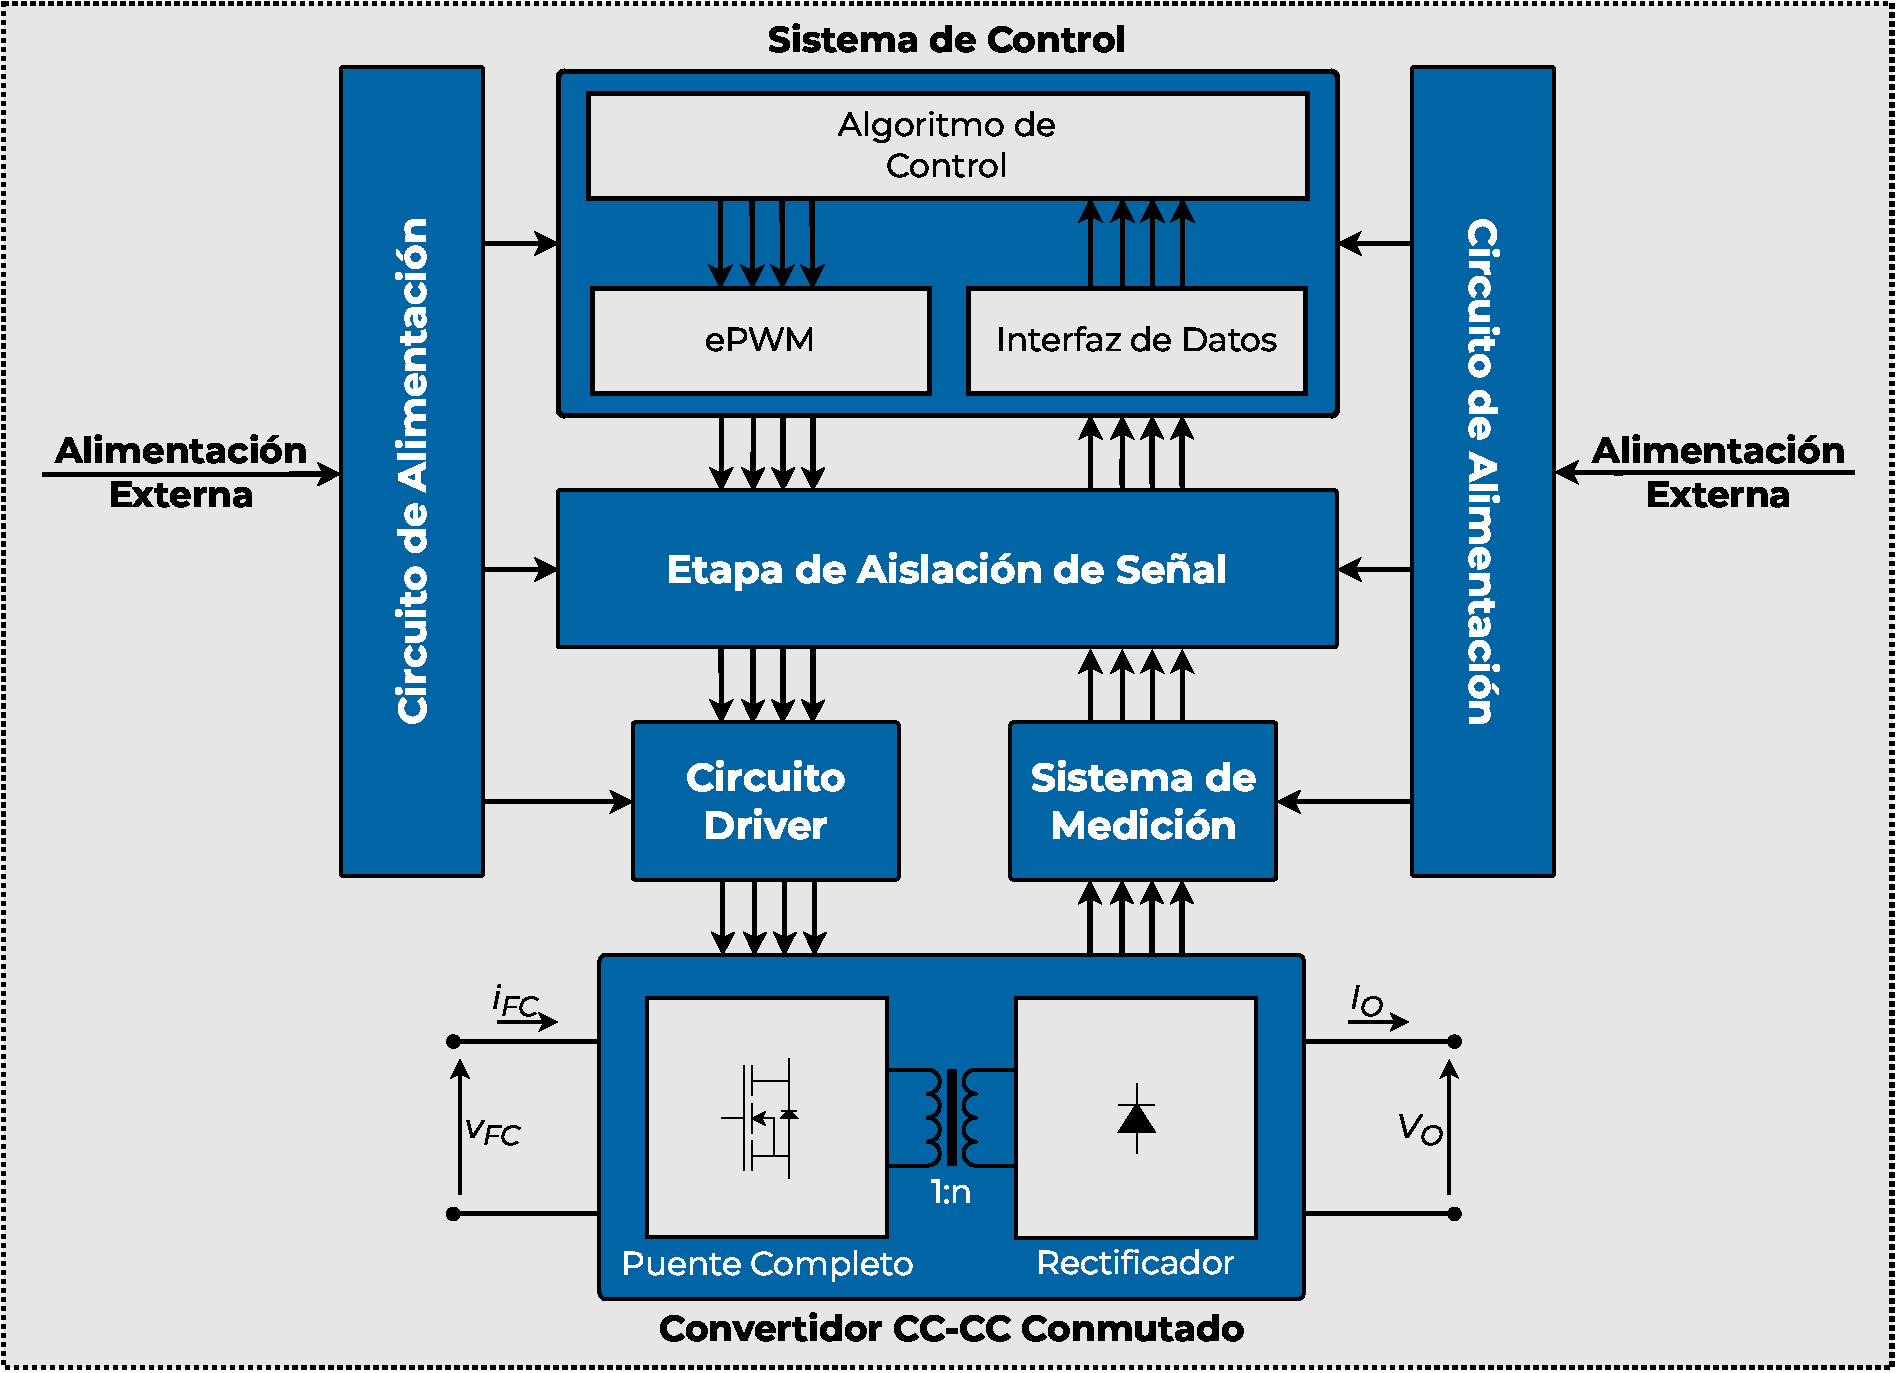
\includegraphics[scale=0.2]{Imagenes/Plataforma Detallada.pdf}
    \caption{Diagrama detallado de la plataforma de evaluación, incluyendo los distintos circuitos auxiliares (Placeholder).}
    \label{diag_detallado}
\end{figure}

Cada uno de estos seis bloques cumplen una función específica que se detalla a continuación:\\

\begin{itemize}
    \item {\SemiBold Convertidor CC-CC Conmutado:} Este es el convertidor de tipo puente completo que se trató en el capítulo anterior. En este capítulo se va a realizar el dimensionamiento de todos sus componentes teniendo en cuenta sus especificaciones. 
    \item {\SemiBold\textit{Driver}:} Este circuito se encarga de entregar la corriente y tensión necesaria para disparar los transistores de potencia y conmutarlos correctamente.
    \item {\SemiBold Sistema de Medición:} Este bloque contiene todos los circuitos y componentes necesarios para realizar las mediciones de todos los parámetros de interés de la plataforma. Esto incluye, además de sensores, los circuitos de acondicionamiento de señal donde se requieran.
    \item {\SemiBold Etapa de Aislación:} Esta etapa se encarga de generar una barrera de aislación eléctrica entre los componentes de potencia y los componentes de señal del circuito.
    \item {\SemiBold Sistema de Control:} Este es el bloque de control que se explicó en el anterior capítulo. Obtiene información de distintos parámetros por medio del sistema de medición, y ejerce la acción de control disparando las llaves mediante el driver.
    \item {\SemiBold Circuito de Alimentación:} Es el circuito que se encarga de proveer las corrientes y tensiones necesarias para los componentes que requieren alguna alimentación externa para funcionar (por ejemplo el controlador digital de señales).\\
\end{itemize}

A lo largo de este capítulo se va a tratar uno por uno el diseño de los circuitos que componen a cada uno de los bloques, utilizando múltiples diseños como referencia (ya sean de otros trabajos de investigación o diseños sugeridos de los propios fabricantes). Se van a eligir y dimensionanar los componentes que forman parte de ellos, hasta obtener un esquemático circuital detallado de la plataforma experimental de evaluación completa.\\

Pero antes de comenzar con el primer bloque, se van a plantear algunas consideraciones y criterios generales que se van a utilizar en el diseño de todos los componentes y circuitos de la plataforma.\\

\newpage

\subsection{Consideraciones Generales}

\subsubsection{Aislación de Tierras}

En toda la plataforma se va a trabajar con tres puestas a tierra distintas y aisladas entre sí: $GND_1$ es la tierra del primario del convertidor, $GND_2$ es la tierra del secundario del convertidor, y $GND_D$ es la tierra de las partes de señal y digitales, como los sensores y el DSC.\\

Esto, si bien agrega una mayor complejidad al diseño, es ventajoso por múltiples razones. Primero, evita la generación de interferencia de modo común entre las tierras del convertidor ($GND_1$ y $GND_2$) que manejan altas corrientes y por lo tanto son más ruidosas; y la tierra de señal $GND_D$ de más bajas corrientes que es más sensible al ruido. Además, dadas las altas corrientes del convertidor, esta separación permite la protección de los circuitos de señal ante picos de corriente y tensión inesperados en la parte de potencia.\\

Es por estas razones que además de la tierra, también los circuitos de señal y potencia se encuentran separados por la etapa de aislación entre potencia y señal. Adicionalmente, las fuentes de alimentación externas se encuentran separadas para los componentes de potencia y señal, manteniendo la aislación deseada.\\

\subsubsection{Selección de Componentes}

En líneas generales, a la hora de elegir un circuito para el diseño de los distintos bloques, si es posible se trata de elegir una solución más integrada (es decir utilizar un circuito integrado que haga esta tarea en vez de diseñar un circuito discreto). Esto simplifica los circuitos y disminuye la cantidad de componentes necesarios a la hora de implementarlos. Además, al estar toda la solución integrada, el rendimiento es más predecible y se encuentra acotado a los parámetros dados por el fabricante del circuito integrado.\\

En todos los casos, se utilizan como guía para el diseño de todas las partes los parámetros de rendimiento y las recomendaciones de diseño especificadas en las hojas de datos  y notas de aplicación de los fabricantes de cada circuito integrado.\\

\subsubsection{Herramientas de Software}

\paragraph{Software EDA}

Para realizar el diseño de todos los esquemas circuitales del sistema, y luego plasmarlos a una placa de circuito impreso se debe utilizar un herramienta de automatización de diseño electrónico o EDA (del inglés \textit{Electronic Design Automation}). Existe una gran variedad de programas que cumplen este propósito, estando entre los más conocidos el \textit{Altium Designer} de \textit{Altium}, el \textit{EAGLE} de \textit{Autodesk}, el \textit{KiCad} y el \textit{Proteus Design Suite} de \textit{Labcenter Electronics}.\\

Para este proyecto se eligió utilizar la plataforma {\Medium KiCad} (que se encuentra en la versión 6.0.7 al momento de escribir este informe), una suite de software libre, gratuita y de código abierto que incluye todas la funcionalidades necesarias para el diseño electrónico. Cuenta con herramientas de captura de esquemático, diseño de PCB, simulación mediante SPICE o Ngspice, visualización de archivos de fabricación y cálculos de diseño de PCB.\\

\begin{figure}[h]
    \centering
    
\includegraphics[scale=0.6]{Imagenes/KiCad.pdf}
    \caption{Logotipo de la plataforma KiCad EDA.}
    \label{logo_kicad}
\end{figure}

El programa también cuenta con una extensa biblioteca de componentes y \textit{footprints} (son las \quotes{huellas} de los componentes en en el circuito impreso) y la capacidad de crear o importar bilbiotecas. Además tiene la capacidad de generar archivos de fabricación, modelos tridimensionales de la PCB y una \textit{bill of materials} (lista de componentes).\\

\paragraph{Software de Simulación}

Para todo lo que se refiere a la simualción de la plataforma; más particularmente las simulaciones del funcionamiento del convertidor CC-CC para su comprensión, estudio, diseño y dimensionamiento; se utilizó la herramienta {\Medium\textit{Simulink}} dentro de la suite de software de \textit{MATLAB-Simulink}.\\

\begin{figure}[h]
    \centering
    
\includegraphics[scale=0.08]{Imagenes/Simulink.png}
    \caption{Logotipo de la plataforma de simulación Simulink.}
    \label{logo_simulink}
\end{figure}

Específicamente, para simulaciones circuitales se hizo uso de el paquete \textit{Simscape Electrical} dentro de Simulink, que permite trabajar con tensiones y corrientes, a diferencia de las herramientas estándar que trabajan con diagramas de bloques.\\

\paragraph{Otras Herramientas}

Adicionalmente, para llevar un control de versiones completo del diseño de la plataforma sobre el que se trabaja, además de mantener un historial completo de todos los cambios, se trabajó con la herramienta de software de control de versiones {\Medium\textit{Git}}.\\

\begin{figure}[h]
    \centering
    
\includegraphics[scale=0.6]{Imagenes/Git.pdf}
    \caption{Logotipo del software de control de versiones Git.}
    \label{logo_git}
\end{figure}

Con este software se crea un \textit{repositorio} donde se almacenan los archivos que se quiere controlar, manteniendo un control de la historia de cada uno de los archivos del repositorio. Para mantener los archivos sincronizados entre varias computadoras y mantener copias de seguridad, se utiliza adicionalmente la plataforma web {\Medium\textit{GitHub}} para hostear el repositorio en la nube, manteniendo una copia segura que se puede copiar a cualquier computadora.\\